\documentclass{article}

\usepackage{authblk}
\usepackage{graphicx}
\usepackage{array}

\title{
    Comunicação por Computador \\
    \large{Trabalho Prático 1}
}
\author{
    Marco Costa A93283
}
\date{27 de outubro de 2021}
\affil{
    Universidade do Minho
}

\begin{document}
        \maketitle
    \section*{Respostas}
        \subsection*{Parte I}
            \subsubsection*{1}
                {
                    \centering
                    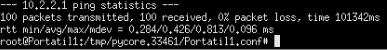
\includegraphics[width=12cm]{images/ping-portatil.png}
                    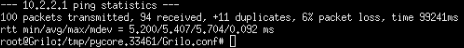
\includegraphics[width=12cm]{images/ping-grilo.png}
                    \par
                }
                    Como podemos ver nas imagens o nó \textit{Grilo}, que no \textit{CORE} lhe foi dada
                uma conexão com 10\% de duplicação e 5\% de packet loss, de 100 pacotes enviados apenas recebeu
                94 mais 11 pacotes duplicados. Isto contrasta com o \textit{Portatil1} que com uma conexão boa conseguiu
                receber os 100 pacotes de resposta sem qualquer duplicação ou perda destes.\par

                    Mais interessante é o resultado destes problemas de conexão no \textit{rtt(round-trip time)} em que se pode verificar
                que o \textit{Grilo} teve valores significativamente mais elevados que a sua contraparte. Apesar disto o \textit{Grilo} demorou
                menos 2101ms a executar.
            \subsubsection*{2}
                {
                    \centering
                    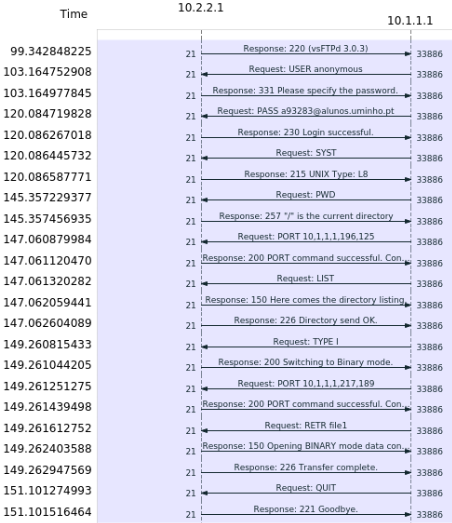
\includegraphics[width=12cm]{images/ftp-flow-graph.png}
                    \par
                }
                    Através do diagrama produzido, pelo wireshark, podemos ver toda a comunicação FTP feita entre o \textit{Portatil1} (10.1.1.1) e o \textit{Servidor1} (10.2.2.1).

		            O início da conexão começa com o envio do tipo de segmento SYN

                    Para além disso, o diagrama mostra que a conexão do lado do servidor está a ser feita na porta 20 que é reservada para o protocolo FTP.
            \subsubsection*{3}
                {
                    \centering
                    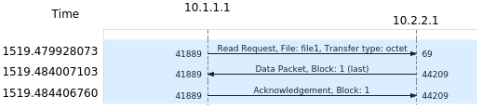
\includegraphics[width=12cm]{images/tftp-wireshark-flow-graph.png}
                    \par
                }
		            Através do diagrama produzido, pelo wireshark, podemos ver toda a comunicação TFTP feita entre o \textit{Portatil1} (10.1.1.1) e o \textit{Servidor1} (10.2.2.1).

                    O protocolo TFTP mostra-se bem mais simples que o FTP tendo sido apenas trocados 3 pacotes, pois utiliza UDP na camada de transporte o que significa que não tem as fases de início e fim de conexão.

                    É feito um \textit{Read Request}, o servidor envia o ficheiro e, por fim, o portátil responde com um \textit{Acknoulegment}.

                    Tal como no exercício anterior podemos conferir no diagrama que o servidor inicia a conexão na porta 69 que corresponde a porta reservada para o TFTP. No entanto, a conexão muda para a porta 44209 para ocorrer a transferência do ficheiro.
            \clearpage
            \subsubsection*{4}
		            Em relação ao uso da camada de transporte, a aplicação TFTP é a única que utiliza UDP. As outras três aplicações utilizam TCP, no entanto versões mais recentes de HTTP utilizam UDP+QUIC.

                    Após o uso dos quatro programas podemos concluir que o mais seguro é o sftp pelo seu uso do protocolo ssh que encripta toda a comunicação entre despositivos. Enquanto que FTP e TFTP não fazem encriptação nenhuma dos dados.

                    Em termos de simplicidade http é o melhor devido ao facto de que só é necessário enviar um pacote \textit{GET} e o servidor retorna o ficheiro.
        \subsection*{Parte II}
            \begin{center}
                \scalebox{0.6}{
                    \large{
                        \begin{tabular}{|m{3.3cm}|m{5cm}|m{5cm}|m{4.5cm}|m{5cm}|}
                            \hline
                            \textbf{Comando usado (aplicação)} & \textbf{Protocolo de Aplicação (se aplicável)} & \textbf{Protocolo de Transporte (se aplicável)} & \textbf{Porta de atendimento (se aplicável)} & \textbf{\textit{Overhead} de transporte em bytes (se aplicável)} \\
                            \hline
                            ping          & icmp   & Não tem & Não tem &  0 \\
                            \hline
                            traceroute    & icmp   & Não tem & Não tem &  0 \\
                            \hline 
                            telnet        & telnet & tcp     & 23      & 20 \\
                            \hline
                            ftp           & ftp    & tcp     & 20,21   & 20 \\
                            \hline
                            tftp          & tftp   & udp     & 69,?    &  8 \\
                            \hline
                            http(browser) & http   & tcp     & 80      & 20 \\
                            \hline
                            nslookup      & dns    & udp     & 53      &  8 \\
                            \hline
                            ssh           & ssh    & tcp     & 22      & 20 \\
                            \hline
                        \end{tabular}
                    }
                }
            \end{center}
\end{document}
